\documentclass[tikz,border=6pt]{standalone}
\usepackage{amsmath,amssymb,mathtools,physics,bm,nicefrac,wasysym}
\usepackage{xcolor}

\definecolor{colone}{RGB}{180,60,60}
\definecolor{coltwo}{RGB}{60,110,180}
\definecolor{colthree}{RGB}{60,140,80}

\definecolor{accent}{HTML}{A13D2C}
\definecolor{accent2}{HTML}{2B5F6B}
\definecolor{muted}{HTML}{5A564F}
\definecolor{panel}{HTML}{F8F6F0}
\definecolor{linecol}{HTML}{D8D2C4}
\definecolor{ink}{HTML}{1E1C1A}
\definecolor{astroblue}{HTML}{1B4F72}
\definecolor{astrodark}{HTML}{17202A}
\definecolor{sunyellow}{HTML}{E8A33D}

\usetikzlibrary{calc,arrows.meta,positioning,decorations.pathreplacing,decorations.markings,angles,quotes,shapes.geometric}
\usepackage{tikz-3dplot}

\newcommand{\vecr}{\vec r}
\newcommand{\vecL}{\vec L}
\newcommand{\vecA}{\vec A}
\newcommand{\vecf}{\vec f}
\newcommand{\vecF}{\vec F}
\newcommand{\vecp}{\vec p}
\newcommand{\avg}[1]{\left\langle #1\right\rangle}
\newcommand{\vecx}{\vec x}
\newcommand{\hatn}{\hat n}
\newcommand{\rhat}{\hat r}
\newcommand{\phihat}{\hat\phi}
\newcommand{\thetahat}{\hat\theta}
\newcommand{\note}[1]{\textcolor{blue!60!black}{\textit{[#1]}}}

% Astronomical acronyms
\newcommand{\LST}{\mathrm{LST}}
\newcommand{\GST}{\mathrm{GST}}
\newcommand{\GMST}{\mathrm{GMST}}
\newcommand{\GAST}{\mathrm{GAST}}
\newcommand{\LMST}{\mathrm{LMST}}
\newcommand{\LAST}{\mathrm{LAST}}
\newcommand{\UT}{\mathrm{UT}}
\newcommand{\UTC}{\mathrm{UTC}}
\newcommand{\TAI}{\mathrm{TAI}}
\newcommand{\TT}{\mathrm{TT}}
\newcommand{\TDB}{\mathrm{TDB}}
\newcommand{\JD}{\mathrm{JD}}
\newcommand{\MJD}{\mathrm{MJD}}
\newcommand{\EoT}{\mathrm{EoT}}
\newcommand{\SNR}{\mathrm{SNR}}
\newcommand{\RON}{\mathrm{RON}}

% Helper commands for specific diagrams
\newcommand{\midlinelabel}[3]{
    \node (midlabel) at ($ (#1)!.5!(#2) $) {#3};
    \draw[stealth-] (#1) --  (midlabel);
    \draw[-stealth] (midlabel) -- (#2);
}
\newcommand{\midlinelabell}[3]{
    \node[fill = white, inner sep = 0.2pt, outer sep=3pt] (midlabel) at ($ (#1)!.5!(#2) $) {#3};
    \draw[stealth-] (#1) --  (midlabel);
    \draw[-stealth] (midlabel) -- (#2);
}
\newcommand{\midlinelabelll}[3]{
    \node[fill = white, inner sep = 0.2pt, outer sep=3pt,scale=0.6] (midlabel) at ($ (#1)!.5!(#2) $) {#3};
    \draw[stealth-] (#1) --  (midlabel);
    \draw[-stealth] (midlabel) -- (#2);
}



\begin{document}
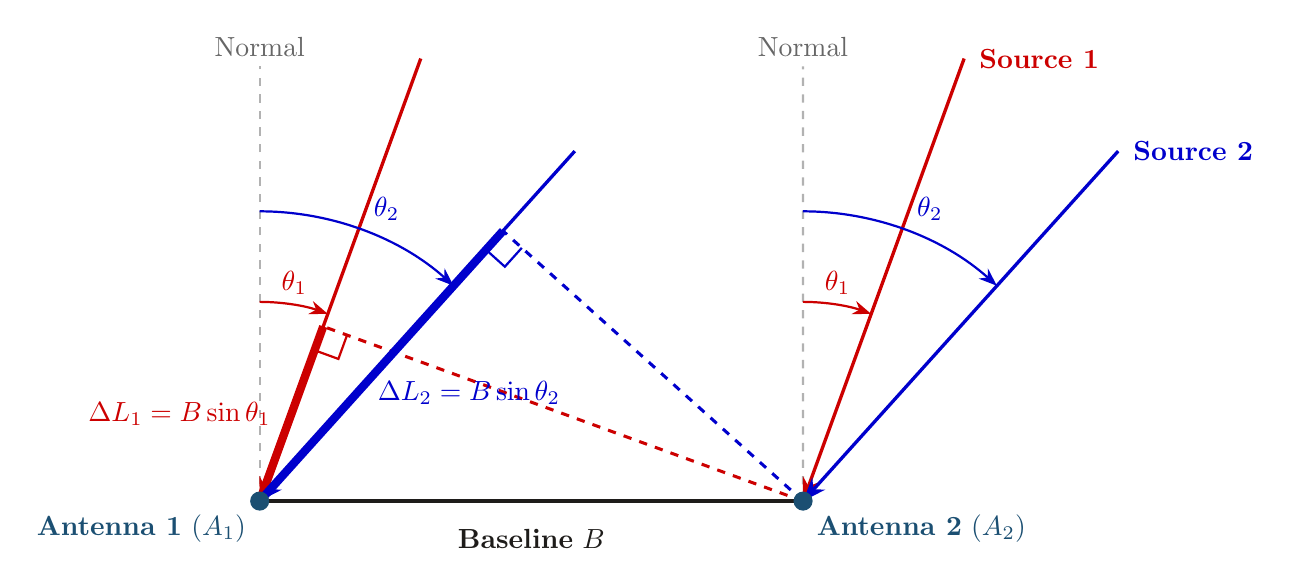
\begin{tikzpicture}[scale=1.15, >=Stealth]
    \def\B{6.0}
    \def\thOne{20}
    \def\thTwo{42}
    \def\rayLen{5.2}
    
    \coordinate (A1) at (0,0);
    \coordinate (A2) at (\B,0);
    
    % Normal lines
    \draw[dashed, gray!60, thick] (A1) -- (0, 4.8) node[above, gray!80!black] {Normal};
    \draw[dashed, gray!60, thick] (A2) -- (\B, 4.8) node[above, gray!80!black] {Normal};
    
    % Source 1 directions (coming from upper right at angle thOne to normal)
    \pgfmathsetmacro{\sOneX}{\rayLen*sin(\thOne)}
    \pgfmathsetmacro{\sOneY}{\rayLen*cos(\thOne)}
    \coordinate (S1_A1) at (\sOneX, \sOneY);
    \coordinate (S1_A2) at ({\B + \sOneX}, \sOneY);
    
    % Source 2 directions (coming from upper right at angle thTwo to normal)
    \pgfmathsetmacro{\sTwoX}{\rayLen*sin(\thTwo)}
    \pgfmathsetmacro{\sTwoY}{\rayLen*cos(\thTwo)}
    \coordinate (S2_A1) at (\sTwoX, \sTwoY);
    \coordinate (S2_A2) at ({\B + \sTwoX}, \sTwoY);
    
    % Intersection points W1 and W2 on ray A1 from wavefronts starting at Antenna 2 (A2)
    \pgfmathsetmacro{\wOneX}{\B*sin(\thOne)*sin(\thOne)}
    \pgfmathsetmacro{\wOneY}{\B*sin(\thOne)*cos(\thOne)}
    \coordinate (W1) at (\wOneX, \wOneY);
    
    \pgfmathsetmacro{\wTwoX}{\B*sin(\thTwo)*sin(\thTwo)}
    \pgfmathsetmacro{\wTwoY}{\B*sin(\thTwo)*cos(\thTwo)}
    \coordinate (W2) at (\wTwoX, \wTwoY);
    
    % Incoming rays for Source 1 (Red)
    \draw[->, very thick, red!80!black] (S1_A1) -- (A1);
    \draw[->, very thick, red!80!black] (S1_A2) -- (A2);
    
    % Incoming rays for Source 2 (Blue)
    \draw[->, very thick, blue!80!black] (S2_A1) -- (A1);
    \draw[->, very thick, blue!80!black] (S2_A2) -- (A2);
    
    % Wavefronts from Antenna 2 (A2) hitting rays at Antenna 1 at exact 90 degrees
    \draw[dashed, line width=1.1pt, red!80!black] (A2) -- (W1);
    \draw[dashed, line width=1.1pt, blue!80!black] (A2) -- (W2);
    
    % Right angle markers at W1 and W2 (exact 90-degree square markers)
    \pgfmathsetmacro{\sqSize}{0.28}
    \draw[thick, red!80!black] 
        ($(W1) + ({\sqSize*cos(\thOne)}, {-\sqSize*sin(\thOne)})$) -- 
        ++({-\sqSize*sin(\thOne)}, {-\sqSize*cos(\thOne)}) -- 
        ($(W1) + ({-\sqSize*sin(\thOne)}, {-\sqSize*cos(\thOne)})$);
        
    \draw[thick, blue!80!black] 
        ($(W2) + ({\sqSize*cos(\thTwo)}, {-\sqSize*sin(\thTwo)})$) -- 
        ++({-\sqSize*sin(\thTwo)}, {-\sqSize*cos(\thTwo)}) -- 
        ($(W2) + ({-\sqSize*sin(\thTwo)}, {-\sqSize*cos(\thTwo)})$);
        
    % Path lags along ray entering Antenna 1
    \draw[line width=3.0pt, red!80!black] (W1) -- (A1);
    \node[left=4pt, red!80!black, font=\bfseries] at ($(W1)!0.5!(A1)$) {$\Delta L_1 = B\sin\theta_1$};
    
    \draw[line width=3.0pt, blue!80!black] (W2) -- (A1);
    \node[right=4pt, blue!80!black, font=\bfseries] at ($(W2)!0.6!(A1)$) {$\Delta L_2 = B\sin\theta_2$};
    
    % Baseline line
    \draw[line width=1.6pt, ink] (A1) -- (A2) node[midway, below=6pt] {\textbf{Baseline} $B$};
    \fill[astroblue] (A1) circle (3pt) node[below left=2pt] {\textbf{Antenna 1} ($A_1$)};
    \fill[astroblue] (A2) circle (3pt) node[below right=2pt] {\textbf{Antenna 2} ($A_2$)};
    
    % Angle arcs at A2
    \draw[->, thick, red!80!black] (\B, 2.2) arc (90:{90-\thOne}:2.2) node[midway, above] {$\theta_1$};
    \draw[->, thick, blue!80!black] (\B, 3.2) arc (90:{90-\thTwo}:3.2) node[midway, above right] {$\theta_2$};
    
    % Angle arcs at A1
    \draw[->, thick, red!80!black] (0, 2.2) arc (90:{90-\thOne}:2.2) node[midway, above] {$\theta_1$};
    \draw[->, thick, blue!80!black] (0, 3.2) arc (90:{90-\thTwo}:3.2) node[midway, above right] {$\theta_2$};
    
    % Source labels at top
    \node[red!80!black, right=2pt, font=\bfseries] at (S1_A2) {Source 1};
    \node[blue!80!black, right=2pt, font=\bfseries] at (S2_A2) {Source 2};
\end{tikzpicture}
\end{document}
